\section{Structure of a Remixing System} 
I plan to study the sociotechnical architecture of the Scratch Online Community by examining its following structural attributes (Figure~\ref{fig:structure}):
1) granularity of the remixable components, 
2) modularity of the remixable components, 
3) decomposability of finished projects, 
4) attributability mechanisms and 
5) openness to remix across systems.

In this proposal I briefly define each structural attribute using one or two examples and I explain how I am planning to go about studying it.
I plan to do analyze these structural properties of the system using varied approaches including:
1) case studies that give an rich description of different scenarios that elucidate on the influence of each attribute,
2) analyses the data corpus to understand the frequency of the scenarios and the relationships between the structural attributes,
3) natural design experiments to study the effect of varying some of the structural dimensions.

\begin{figure}
\centering
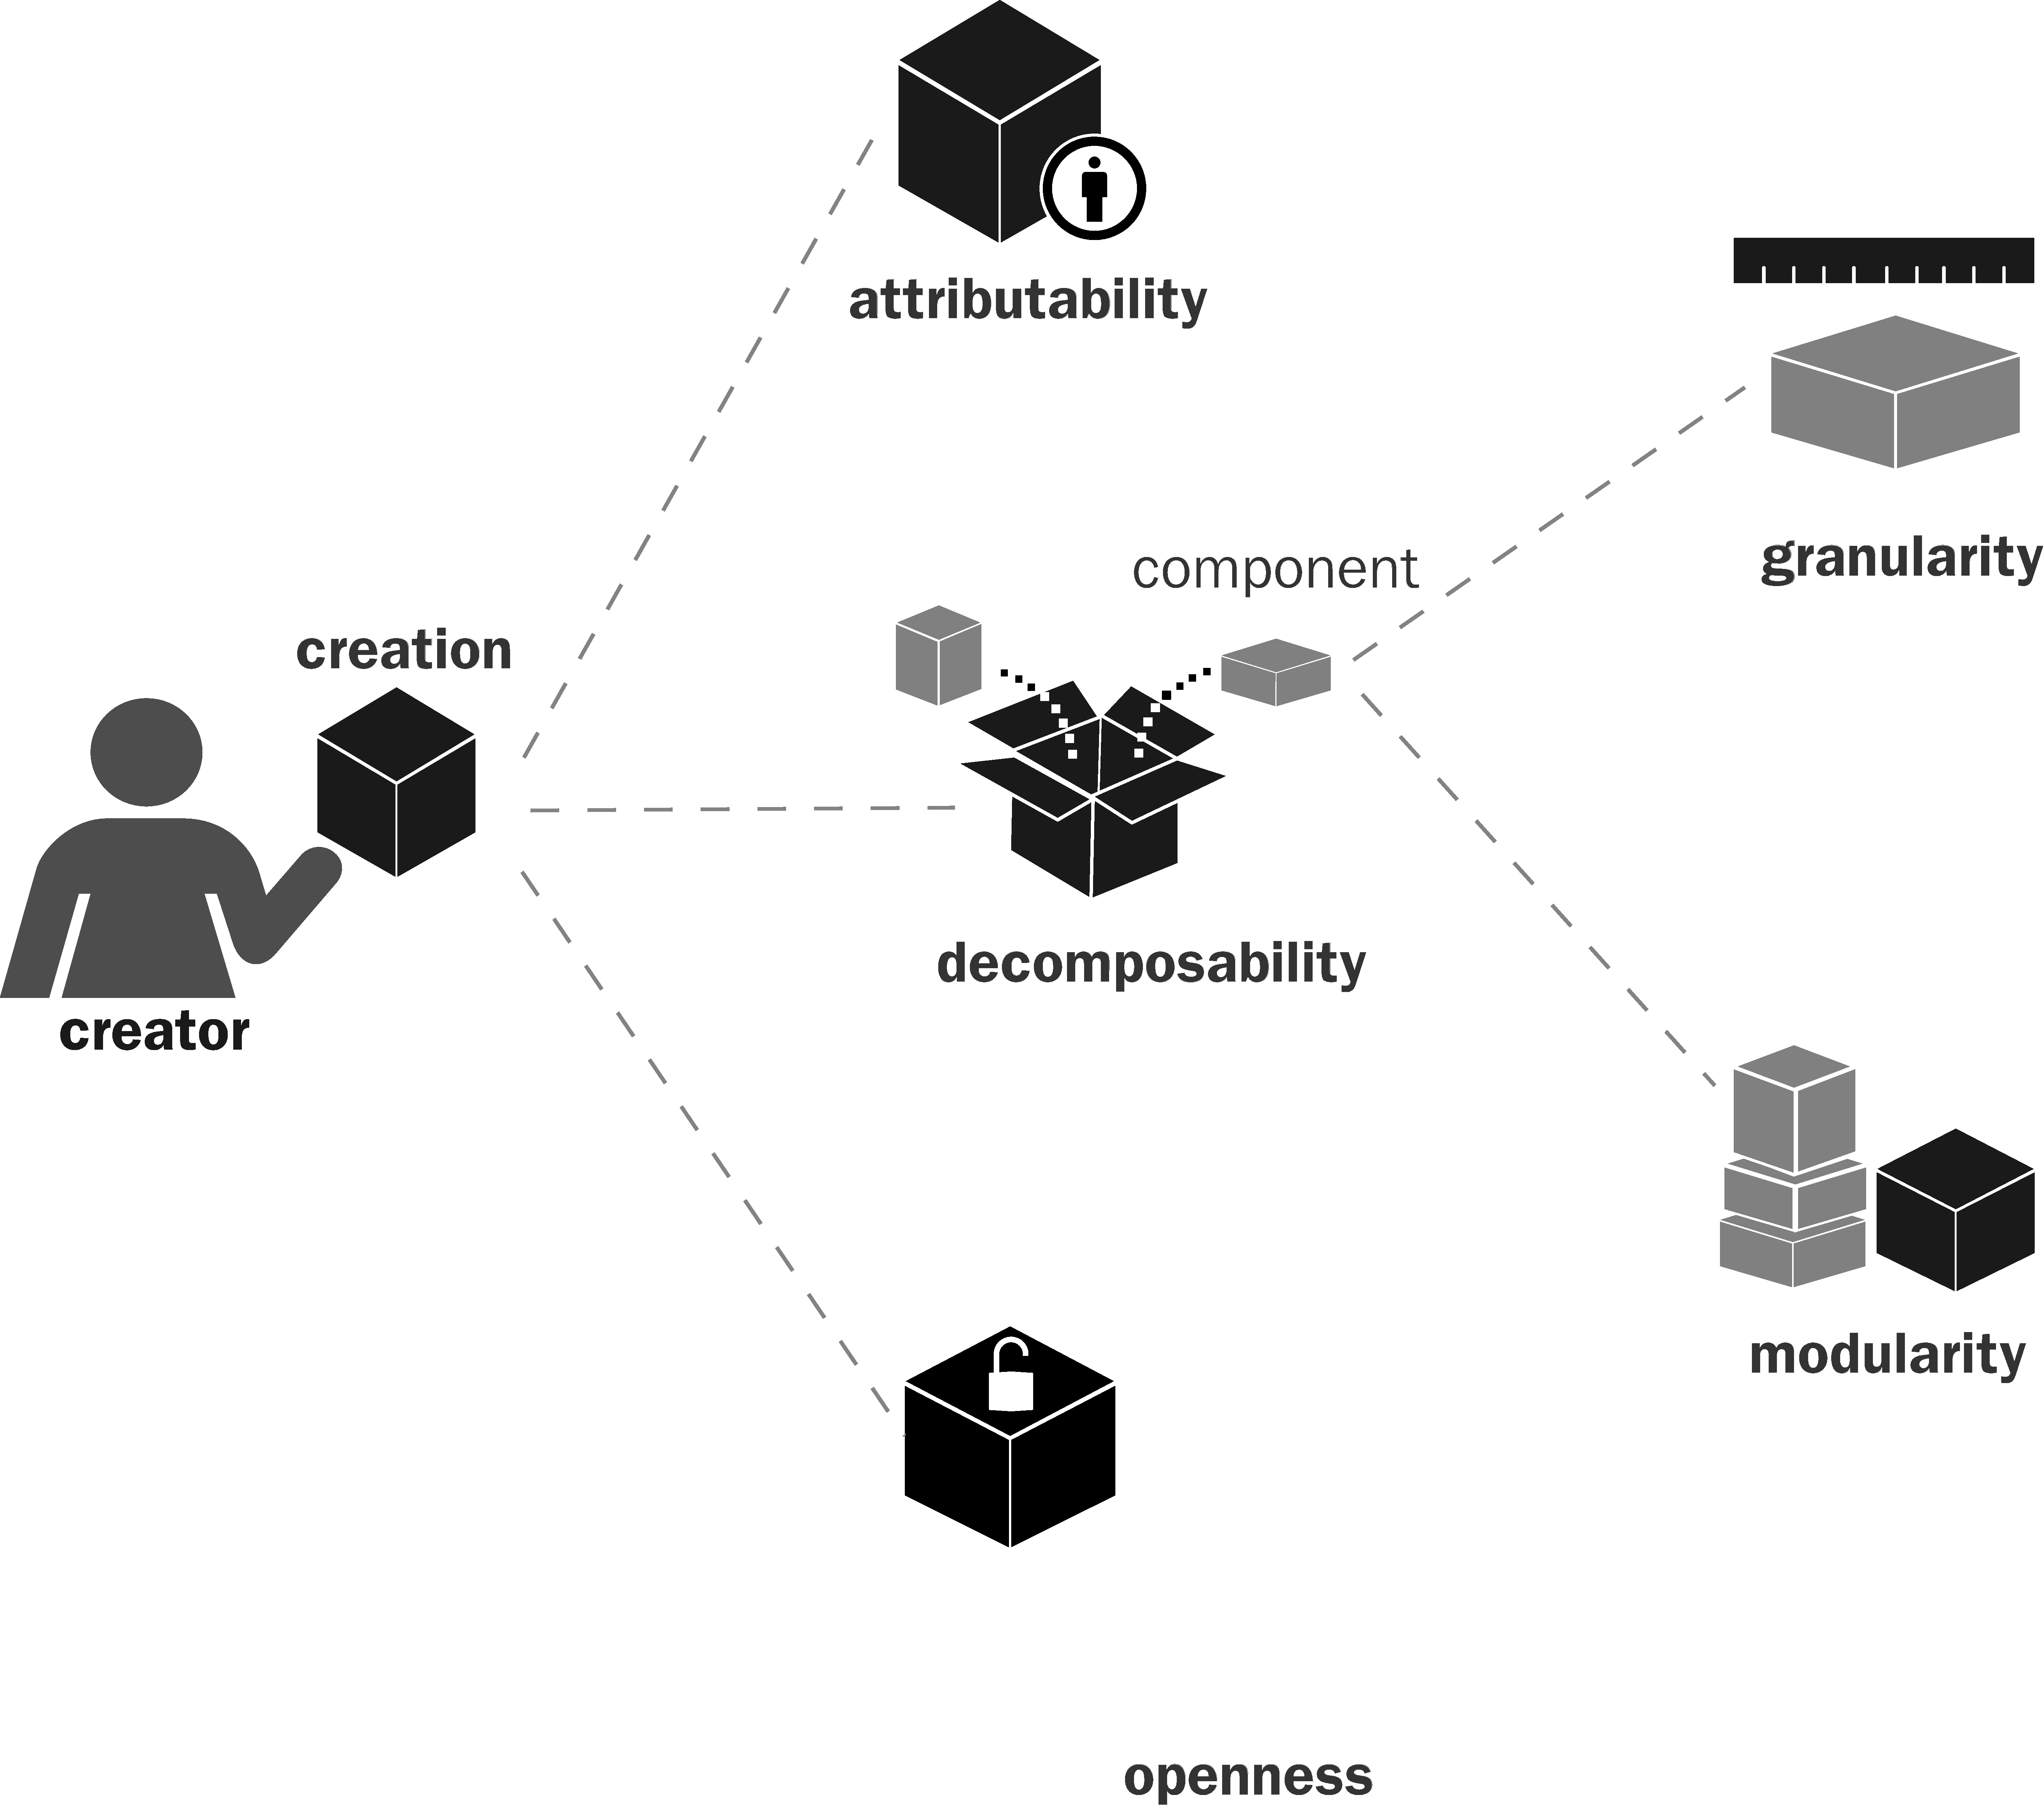
\includegraphics[width=3.25in]{figures/structure.pdf}
\caption{Structural dimensions of a remixing system}
\label{fig:structure}
\end{figure}

\subsection{Granularity}
Granularity is the size of projects' modules \citet{benkler_coases_2002}. 
In Scratch, projects have a couple levels of granularity.
Projects are made up of ``sprites'', for example, characters in a game or a elements in the user interface elements of an interact simulations.
Each sprite can have ``scripts'' or  stacks of programming blocks that control the sprite's behavior such as its position on the screen, its looks, sounds and interaction with other sprites and the user (via mouse, keyboard, or other sensors).
Each sprite also has one or more costumes or images that represent the different visual states of a sprite.
Sprites can also have sounds that are played programmatically, for example, a character in a game could make a sound each time it jumps.

\subsubsection{Proposed work}
The Scratch Online Community, by default it only allows for sharing at the coarsest degree of granularity: only projects can be shared. 
I plan to analyze the implications of this design decision and the ways  people get around the limitations of the architecture.

I have anectdotal evidence that Scratch participants get around the granularity limitations by sharing full projects with the sole intention of sharing a single sprite, script, image or sound.
This need for finer granularity often stems from a desire to engage in sharing practices that the original design did not anticipate. For example, I have documented before the existence of ``coloring contests'' \citep{nickerson_appropriation_2011} where Scratch community remix in order to add color to an image. or as part of group collaboration.
I plan to look these practices in more detail to understand the ways in which a finer granularity mechanisms would help support different types of creative and collaborative learning practices beyond the the existing research that suggests that finer granularity is correlated to the number of people engaged in cooperative activities.

In order to analyze the effect of explicitly supporting finer degree of granularity through a natural experiment, I plan to analyze the adoption ``Scratch Resources'' \footnote{Available at http://resources.scratchr.org}, a website created by members of the Scratch community to support sharing sprites, images and sounds. 

Some of my motivating questions are: 
how common is sharing and remixing across the different levels of granularity available (even if not explicitly supported)?
what are the types of participants and motivations for sharing finer grained components?
what role does granularity play in the likelihood of a project being remixed controlling for all other factors?
how do different levels of granularity impact the type and quality of remixes?
how do different levels of granularuty support different levels of familiarity with Scratch, that is, are novices more likely to rely on coarser granularity when engaging in remixing as a scaffolding mechanism?

\subsection{Modularity}
\citet{benkler_coases_2002} defines modularity as the ``property of a project referring to the extent to which it can be broken down into smaller components, or modules, that can be independently and asynchronously produced before they are assembled into a whole.''
For the purpose of this work, I will separate the two aspects of modularity described above by separating what happens before and after a project is shared:
a) the ease of \emph{decomposing} an already shared project into smaller components and 
b) the ease of \emph{remixing and integrating} such components into new creations.

In this section of the analysis, I plan to frame the analysis of ``modularity'' by focusing on the ``ease of remixing'' a component such as a sprite, script, image or sound. 
The next section will focus on the ease of decomposing a compiled project.

I plan to analyze this by examining the attributes of remixed components. 
I will start by analyzing the sample components that come pre-installed with Scratch.
For example, Scratch comes with a sprite called ``jetpack girl'' which consists of five costumes and five sounds of a flying character that can be controlled with the keyboard.
The code of the sprite comes with an invitation to remix: ``Import me into your own project'' and an explanation on how to use it ``arrow keys make me fly''.
This sprite has been remixed several times.
I intend to analyze the set of sprites, images and sounds that come with Scratch and study how modular they are by looking at how often and it what ways they get remixed.
I plan to analyze the ways different modules are remixed, the types of users who do so and at what point in their Scratch life they do remix them.
I then plan to analyze components that are generated by the community.


% 2. modularity: both technical and sociocultural. 
% Description:
% For example, a ball that has gravity implemented in it, can be easily repurpiosed while a complicated interconnected set of sprites and scipts in a complexly prorgammed projects are much harder to detach and modularized. 
%
% Example: 
% - Samples: sample sprites
% - Necklace: physics simulation of a string turned into a necklace. Alterative less modular version: images generated by code.
% - MHM, MakiTak: cultural modularity, reused in multiple scenarios
%
% Proposed work:
% - Look at cultural and technical modularity
% - Most modular pieces are those most remixed? Not most modular projects?
% - More modular, less learning?
% - More modular, more used?
% - Individual differences approaches to modularity: cut

\subsection{Decomposability}
% 3. decomposability.
% One of the differences between digital media and its predecesors is that it is often possible to break apart a digital creation into its components. This decomposability is not always possible however. In some cases, there are technical or legal barriers to doing so. For example, a video on YouTube is not easy to decompose into the parts that were used to making it before the editing since the source files are not uploaded while on sites like Aviary, an image can be taken apart in all its compoonents used. With software this issue has been at the forefront of the Free Software movement that advocates for complete decomposability via providing the source code along with its compiled version. 
% Using Scratch as the place to study this, we can observe that projects can be decomposed to its original parts except for its images and sounds that once.
% Rasterization, no layers, no vectors.
% Code is all decomposable to its smallest form which is the blocks.
% Analysis of decomposability of remixes. 
% Practices to prevent decomposing: obfuscation. Anti-remixing. 
% Decomposability is enforced.
% People want to share compiled code but not its components.

\subsection{Attributability}
% Experiments with automatic vs credit. Responses. Results. Previous work. Future work:
% Not always desired attribution.
% - Notes 
% - Creator endorsed attribution.

\subsection{Openness}
% Across systems. Ethos explained. Creative commons version for kids. DeviatnArt conflicts
% 

